\documentclass[11pt, twoside, reqno]{book}
\usepackage{amssymb, amsthm, amsmath, amsfonts}
\usepackage{graphicx}
\usepackage[citation-order]{amsrefs}
\usepackage{color}
\usepackage{hyperref}
\usepackage{verbatim}
\usepackage[title]{appendix}
\usepackage{pdfpages}
\usepackage{bardtex}

\styleoption{seniorproject}


\begin{document}

%For senior projects:
\titlepg{Don't Take This Personally: Sentiment Analysis for Identification of ``Subtweeting" on Twitter}{Noah Segal-Gould}
    {May}{2018}

\abstr

The Oxford English Dictionary states that ``subtweet" is defined as ``(on the social media application Twitter) a post that refers to a particular user without directly mentioning them, typically as a form of furtive mockery or criticism." Following the rapid growth and adoption of social networking websites like Twitter, sentiment analysis has garnered much research interest in recent years. To computationally identify and categorize opinions expressed in text, sentiment analysis of figurative language such as irony and sarcasm has garnered even more recent interest. In this project, I will treat the identification of subtweets as a sentiment analysis problem and utilize a novel approach for data collection and labeling, as well as Naive Bayes text classification. By identifying subtweets as they are posted online in real time, I will create a Twitter bot which archives and interacts with them. In addition to the paper, this project will be made available online with its source code and all data collected during its completion.

\tableofcontents

\dedic

I dedicate this senior project to @jack, who has willfully made numerous changes to Twitter which inevitably angered millions.

\acknowl

Thank you professors Sven Anderson, Keith O'Hara, and Rebecca Thomas for making this project possible through your combined efforts to teach and advise me. Thank you Benjamin Sernau '17 for enduring through three years of Computer Science courses with me and being a source of unending joy in my life. Thank you to Julia Berry '18, Aaron Krapf '18, and Zoe Terhune '18 for being my very best friends and giving me things worth caring about. Finally, thank you to my parents Tammy Segal and Emily Taylor for your constant support and patience throughout my four years at Bard College. 

\startmain


\intro

\section{Background}
\label{background}

The news and social networking service Twitter had over 140 million active users who sent 340 million text-based Tweets to the platform every day by March of 2012  \cite{twitter_stats}. Since Twitter-founder Jack Dorsey sent the first Tweet in March of 2006  \cite{first_tweet} social scientists, advertisers, and computer scientists have applied machine learning techniques to understand the patterns and structures of the conversations held on the platform. One such technique is sentiment analysis, which seeks to ascertain the opinions of bodies of text. Sentiment analysis techniques are often treated as classification problems which seek to place text into categories such as \textbf{positive}, \textbf{negative}, and \textbf{neutral}.

On Twitter, the most common way to publicly communicate with another user is to compose a tweet and place an ``@" before the username of that user somewhere in the tweet (e.g. "How are you doing, @NoahSegalGould?"). Through this method, public discussions on Twitter maintain a kind of accountability: even if one were to miss the notification that they were mentioned in a tweet, one's own dashboard keeps a running list of their most recent mentions. 

If an individual sought to disparage or mock another, they could certainly do so directly. But the targeted user would probably notice, and through the search funtions of the platform, anyone could see who has mentioned either their own or another's username. Instead, a phenomenon persists in which users of the platform deliberately insult others in the vaguest way possible. Tweets of this kind are colloquially called ``subtweets" and typically target a specific person but do not contain the username of that person.

All users do not necessarily possess the same exact definition of ``subtweet." I trust the Oxford English Dictionary's ``[tweet] that refers to a particular user without directly mentioning them, typically as a form of furtive mockery or criticism," however that definition is perhaps too restrictive. Some individuals believe subtweets abide by this definition, but others expand it to allow inclusion of others' real names (especially if that individual does not own a Twitter account), and some do not even require that a particular user be the target of the tweet. In this project, I implement a classifier which abides by a particularly loose definition in order to please as many parties as possible. 

\section{Motivation}
\label{motivation_and_prior_work}

The inspiration for this project came from interests I garnered taking courses within Bard College's Computer Science department as well as its Experimental Humanities concentration. The very first course I attended at Bard College was Professor Keith O'Hara's \textit{Object-Oriented Programming with Robots}. It served as my first introduction to computer programming, and for my final project I created \textit{Fuzzfeed}: a Twitter bot which generated fake \textit{Buzzfeed} article titles. The following academic year, I wrote programs in Professor Collin Jennings' \textit{Signs and Symbols: Patter Recognition in Literature and Code} and Professor Rune Olsen's \textit{Cybergraphics} which analyzed and visualized topic models of poetry on Twitter. The first time I implemented sentiment analysis on my own was in Professor Gretta Tritch-Roman's \textit{Mapping the 19th Century City}, for which I sought to analyze 1860s New York City newspapers for their sentiments toward immigration. Natural language processing struck me as entertaining and fruitful, so I chose to pursue it further.

By my Junior year, my friends and I used Twitter on a daily basis. In my free time, I made Twitter bots that utilized Markov chains to generate text based on corpora of their tweets. Data collection became a passion of mine as I learned to appreciate the utility and acknowledge the deliberate limitations of web-based APIs. I taught myself web-scraping and utilized Python's \textit{BeautifulSoup} library to programmatically acquire text from Bard College's official online course catalog as well as Twitter's web interface. These skills for programmatically interacting with the world wide web became useful resources during the completion of this project.

My peers introduced me to subtweeting, and I started to pay closer attention to tweets that followed the typical patterns of distanced criticism that subtweets were known for. Because some format seemed to exist which was popularly applied to produce the optimal subtweet, I pitched the concept of subtweet classification to my senior project adviser, Professor Sven Anderson, and I started work on this project in the Fall.

I was initially motivated to complete a senior project on this topic because I wanted to create something useful to my peers and also challenge their notions of public and private interactions on social networking applications like Twitter. Individuals I knew personally would take to the platform to complain indirectly about one another through their subtweets. Friends and I shared evenings debating on if a particular mutual friend's complaints were actually subtweets, and I wondered if that guess-work could be done by a program. I also wanted to challenge the hypocrisy of utilizing a service which presents itself as a public forum to speak in distinctly private ways. Toward this end, I decided the project would be in pursuit of the following goals: it would provide a framework for collecting examples of subtweets, train a classification algorithm using those examples, and finally utilize that classifier in real time to make tweets which were intended to be unseen by specific parties easily accessible to all parties. In presenting covertly hurtful content as obviously hurtful in a public fashion, perhaps I could promote a particular awareness that tweets posted by public accounts were indeed publicly accessible, and that Twitter's End User License Agreement (EULA) allowed for this kind of monitoring. 

\section{Literature Review}
\label{literature_review}

Instead of focus groups, opinion polls, and conduct surveys, sentiment analysis and opinion mining programs are increasingly applied to social networking websites to analyze the sentiments and opinions of users toward topics and products. For the Twitter social networking platform, sentiment analysis allows administrators to enforce their hateful conduct policies \cite{hateful_conduct} which specifically prohibit violent threats and some types of degrading content. Sentiment analysis has been utilized for prediction of financial markets \cite{sentiment_analysis_markets} as well as reactions to terrorist attacks \cite{sentiment_analysis_terrorism}, and sentiment analysis with a specific focus on figurative language such as irony has also attracted recent research interest \cite{sentiment_analysis_irony}. In an attempt to mock, subtweets often exhibit figurative language such as irony and hyperbole.

``Subtweet" was coined in December of 2009 by Twitter user Chelsea Rae \cite{first_subtweet} and was entered into Urban Dictionary the following August \cite{urban_dictionary}. In ``To tweet or ‘subtweet’?: Impacts of social networking post directness and valence on interpersonal impressions" \cite{subtweets_communications}, Edwards and Harris sought to analyze student participants' perceptions of known subtweets. In the news, too, subtweets have garnered attention in \textit{The Atlantic} \cite{the_atlantic}, \textit{The Washington Post} \cite{the_washington_post}, and \textit{Slate} \cite{slate}. Despite this recent interest, little to no research exists on applying sentiment analysis to subtweets.

\section{Changes in Data Acquisition}
\label{changes_in_data}

The novel approach I developed for creating a ground truth dataset relied on a particular phenomenon in which Twitter users were already calling-out the subtweets of their peers. The format I noticed followed that a user would post a subtweet which was easily recognized by a peer, and that peer would then reply to that tweet in order to complain that the original user was subtweeting or to ask if the tweet was indeed a subtweet. Initially, the Python script I wrote to utilize the Twitter API's search functionality via the Tweepy library specifically searched for replies to tweets which contained some form of the string ``subtweet" and then utilized the API's status object to access the tweet to which it was replying. Both the alleged subtweet and the tweet containing the accusation were saved to a comma-separated values (CSV) file. I ran the script every day for over two months.

Initially, I trained the classifier using a dataset which was half comprised of these alleged subtweets and half comprised of tweets randomly selected from a dataset provided by Alec Go \cite{go_dataset}. That was a mistake. I had failed to make the training data representative of actual subtweets and non-subtweets. To rectify this, I revised the alleged subtweets downloading script and created one that had the opposite effect: it downloaded tweets with replies which specifically did \textbf{not} contain the string ``subtweet." In both the script which downloaded subtweets and the script which downloaded non-subtweets, I knew my assumptions about these interactions would not hold true in every case. They were intended as generalizations which would make acquiring a ground truth dataset for use in performing binary classification significantly easier and less time-consuming than finding and labeling subtweets and non-subtweets by hand.

\section{The Twitter API}
\label{twitter_api}

[Explain how it is accessed and its limitations.]

\section{Regular Expressions, N-Grams, \& Tokenization}
\label{regular_expressions_etc}

[Explain the use for regular expressions in identifying hashtags, URLs, and mentions.]

[Explain N-Grams and how they help a classifier.]

[Explain tokenization and specifically NLTK's TweetTokenizer.]

\section{TF \& TF-IDF}
\label{tf_tf_idf}

TF-IDF, or term frequency-inverse document frequency, is a statistical representation of how important a single word is for each document in a collection of documents.

[Explain vectorization and provide examples.]

\section{Naive Bayes}
\label{naive_bayes}

Naive Bayes classifiers are probabilistic supervised learning models which make the "naive" assumption of independence between pairs of features being classified. Sentiment analysis is popularly performed through Naive Bayes.

[Explain some probability, the independence assumption, and the multinomial distribution. Give examples.]

\section{Statistical Considerations}
\label{statistical_considerations}

In tasks pertaining to text classification, like sentiment analysis, precision refers to the number of correctly labeled items which were labeled as belonging to the positive class and in fact did belong to that class (true positives) divided by the total number of elements which were labeled as belonging to the positive class including ones which were labeled positively either correctly or incorrectly. Recall, then, refers to the true positives divided by the total number of elements that actually belong to the positive class.

[Explain F1, Precision, Recall, Accuracy, and Null Accuracy.]

\chapter{Implementation}
\label{implementation}

\section{Searching for Tweets Using the Twitter API}
\label{searching_with_api}

[Show code and explain how searching works with Tweepy.]

\section{Cleaning the Data}
\label{cleaning_data}

[Show code and explain how text cleaning genericizes certain features and ignores tweets lacking enough English words.]

\section{Training the Classifier \& K-Folds Cross-Validation}
\label{training_and_k_folds}

[Explain how pipelines are trained and how K-Folds splits the dataset.]

\chapter{Results}
\label{results}

\section{Distributions \& Datasets}
\label{distributions_and_datasets}

[Explain the tables and figures.]

\section{Confusion Matrices}
\label{confusion_matrices}

A confusion matrix is a table which visualizes the performance of an algorithm. In this case, I implemented a Naive Bayes classifier from Scikit Learn on my dataset and included in my results is a confusion matrix of the performance...

[Explain how to read a confusion matrix and show the test and training figures.]

\section{Most Informative Features}
\label{most_informative_features}

[Explain how to read the most informative features for each class (or just the "subtweet" class) and show the table.]

\section{Statistical Analysis}
\label{statistical_analysis}

[Show the scores from K-Folds.]

\section{The Twitter Bot}
\label{the_twitter_bot}

[Explain how the Twitter bot works and show code as well as examples of interactions.]

\chapter{Conclusion}
\label{conclusion}

\section{Summary of Project Achievements}
\label{summary}

[Ground truth data, classifier, cleaning, Twitter bot.]

\section{Future Work \& Considerations}
\label{future_work_and_considerations}

[Test other classification algorithms. Utilize more training data.]

\begin{bibliog}

\bib{twitter_stats}{article}{
	author={Inc., Twitter},
	title={Twitter turns six},
	date={2012},
	eprint={https://blog.twitter.com/official/en_us/a/2012/twitter-turns-six.html},
}

\bib{first_tweet}{article}{
	author={Dorsey, Jack},
	title={inviting coworkers},
	date={2006},
	eprint={https://twitter.com/jack/status/29},
}

\bib{hateful_conduct}{article}{
	author={Twitter},
	title={Hateful conduct policy},
	date={2018},
	eprint={https://help.twitter.com/en/rules-and-policies/hateful-conduct-policy},
}

\bib{sentiment_analysis_markets}{article}{
	author={Nassirtoussi, Arman~Khadjeh},
	author={Aghabozorgi, Saeed},
	author={Wah, Teh~Ying},
	author={Ngo, David Chek~Ling},
	title={Text mining for market prediction: A systematic review},
	date={2014},
	journal={Expert Systems with Applications},
	volume={41},
	number={16},
	pages={7653\ndash 7670},
}

\bib{sentiment_analysis_terrorism}{article}{
	author={Burnap, Pete},
	author={Williams, Matthew~L},
	author={Sloan, Luke},
	author={Rana, Omer},
	author={Housley, William},
	author={Edwards, Adam},
	author={Knight, Vincent},
	author={Procter, Rob},
	author={Voss, Alex},
	title={Tweeting the terror: modelling the social media reaction to the
		woolwich terrorist attack},
	date={2014},
	journal={Social Network Analysis and Mining},
	volume={4},
	number={1},
	pages={206},
}

\bib{sentiment_analysis_irony}{article}{
	author={Reyes, Antonio},
	author={Rosso, Paolo},
	title={On the difficulty of automatically detecting irony: beyond a
		simple case of negation},
	date={2014},
	journal={Knowledge and Information Systems},
	volume={40},
	number={3},
	pages={595\ndash 614},
}

\bib{first_subtweet}{article}{
	author={Rae, Chelsea},
	title={I hate when i see people...},
	date={2009},
	eprint={https://twitter.com/Chelsea_x_Rae/status/6261479092},
}

\bib{urban_dictionary}{article}{
	author={Dictionary, Urban},
	title={Subtweet},
	date={2010},
	eprint={https://www.urbandictionary.com/define.php?term=subtweet},
}

\bib{subtweets_communications}{article}{
	author={Edwards, Autumn},
	author={Harris, Christina~J},
	title={To tweet or ‘subtweet’?: Impacts of social networking post
		directness and valence on interpersonal impressions},
	date={2016},
	journal={Computers in Human Behavior},
	volume={63},
	pages={304\ndash 310},
}

\bib{the_atlantic}{article}{
	author={Madrigal, Alexis~C.},
	title={Behind the machine's back: How social media users avoid getting
		turned into big data},
	date={2014},
	eprint={https://goo.gl/h36jxx},
}

\bib{the_washington_post}{article}{
	author={Dewey, Caitlin},
	title={Study confirms what you always knew: People who subtweet are
		terrible},
	date={2016},
	eprint={https://goo.gl/SeV3mx},
}

\bib{slate}{article}{
	author={Hassler, Chelsea},
	title={Subtweeting looks terrible on you. (you know who you are.)},
	date={2016},
	eprint={https://goo.gl/NCz27z},
}

\bib{go_dataset}{article}{
	title = {Twitter Sentiment Classification using Distant Supervision},
	author = {Go, Alec},
	author = {Bhayani, Richa},
	author = {Huang, Lei},
	journal = {CS224N Project Report, Stanford},
	pages = {12},
	date = {2009}
}

\end{bibliog}

\begin{appendices}

\chapter{subtweets\_downloader.ipynb}
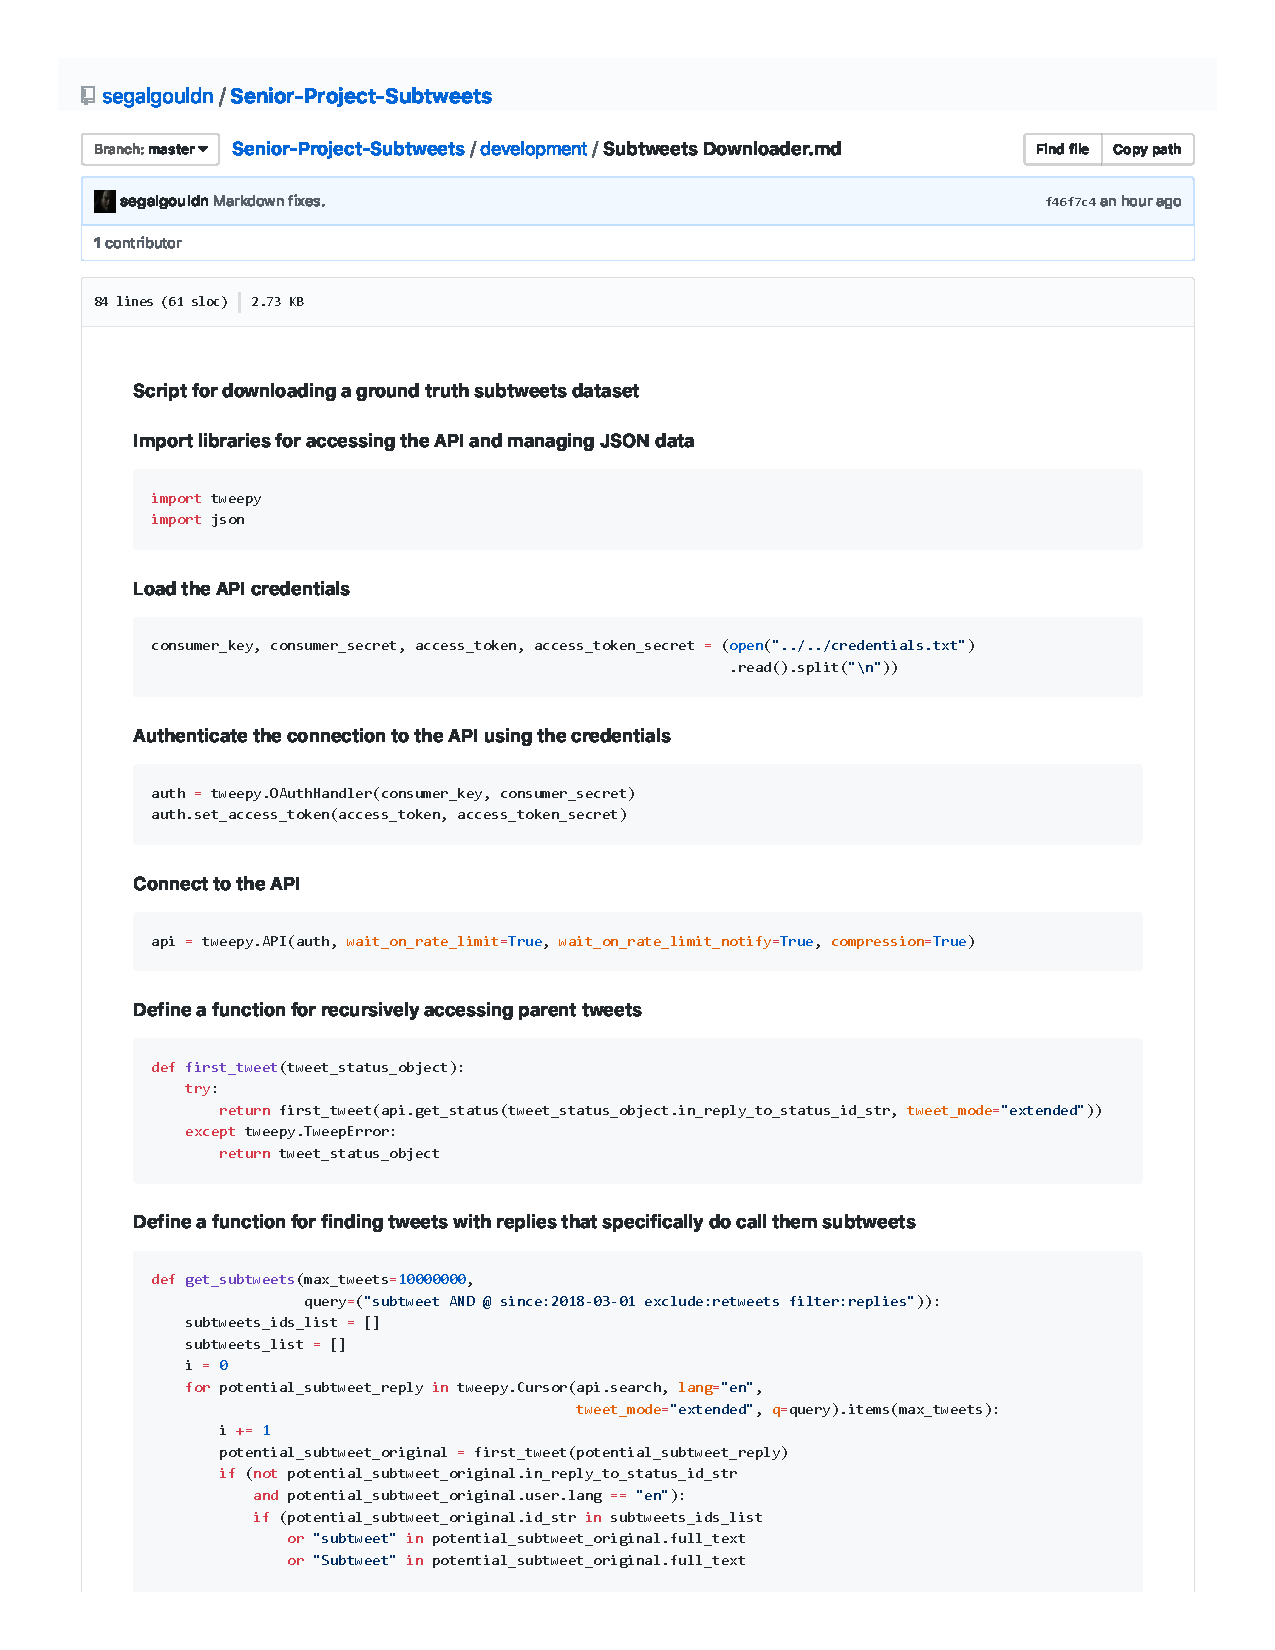
\includepdf[pages=-]{../subtweets_downloader.pdf}

\chapter{non\_subtweets\_downloader.ipynb}
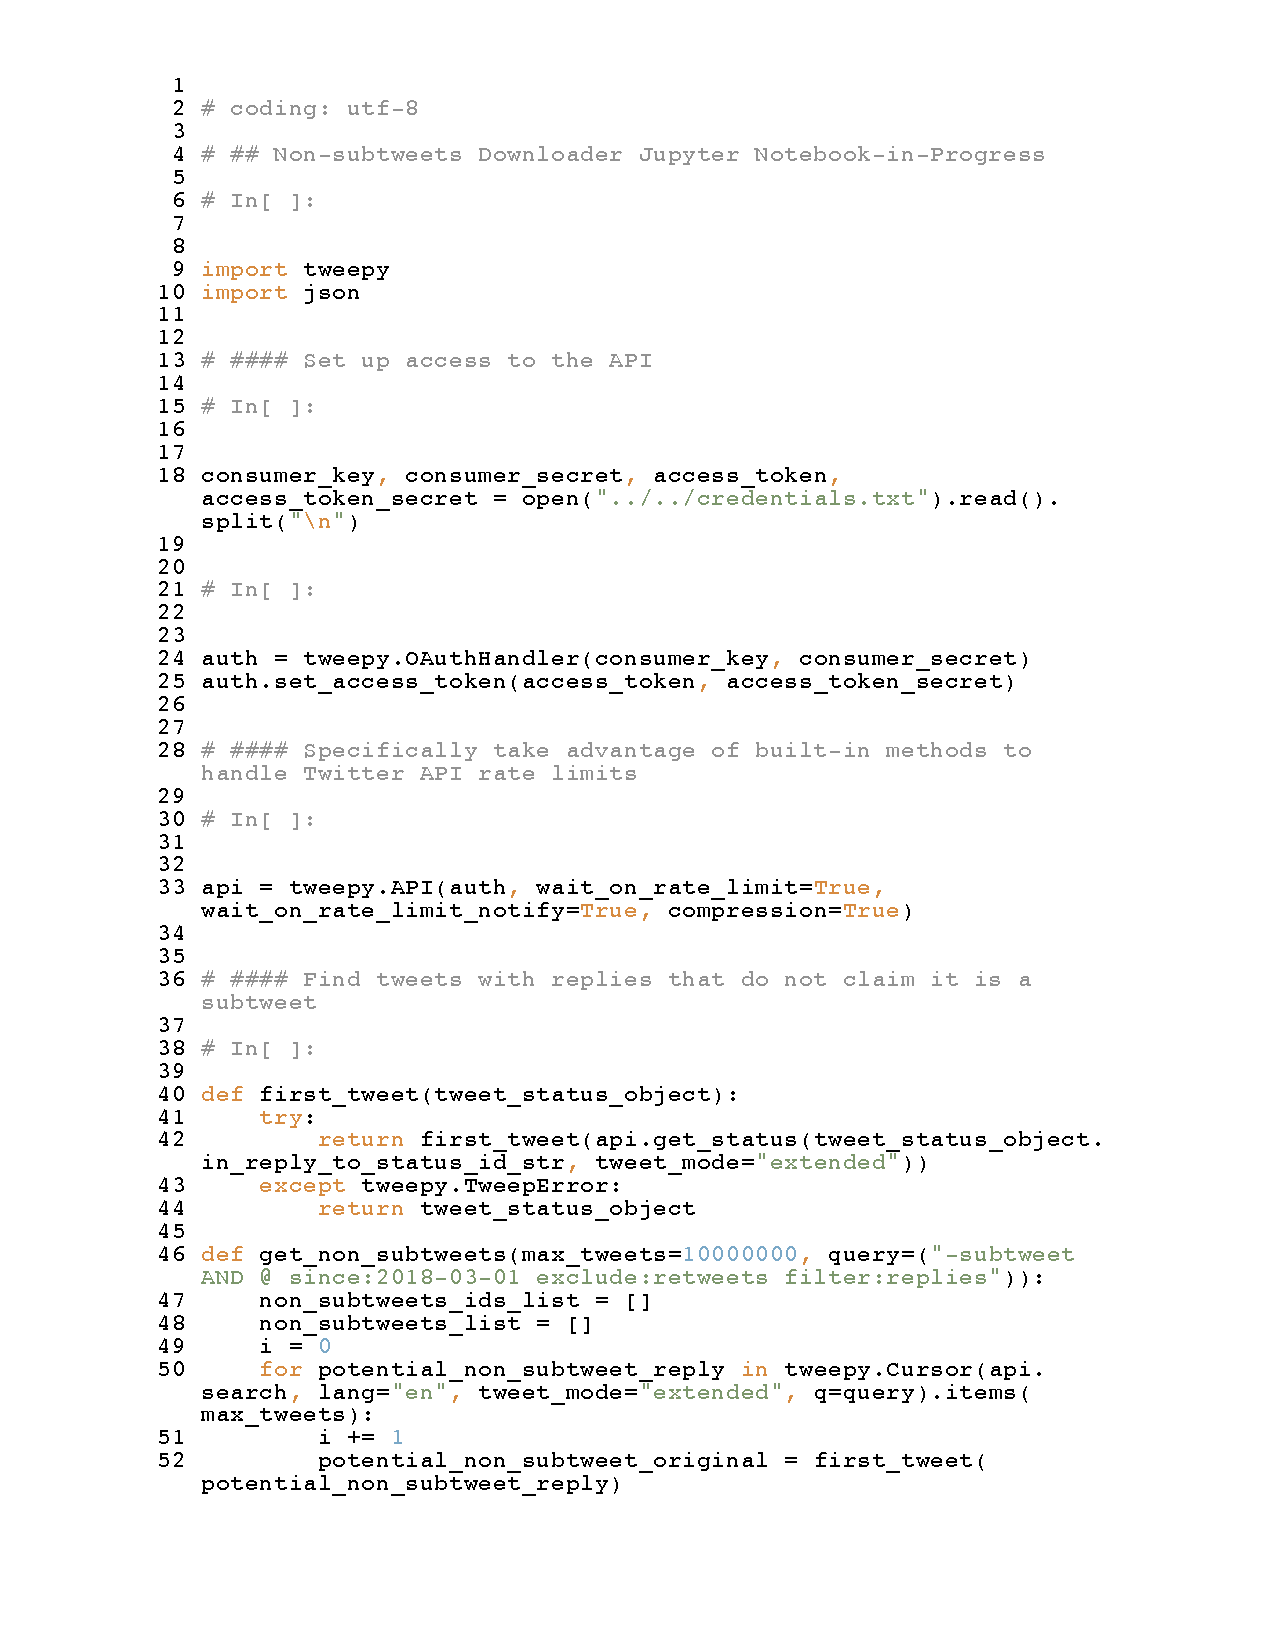
\includepdf[pages=-]{../non_subtweets_downloader.pdf}

\chapter{classifier\_creator.ipynb}
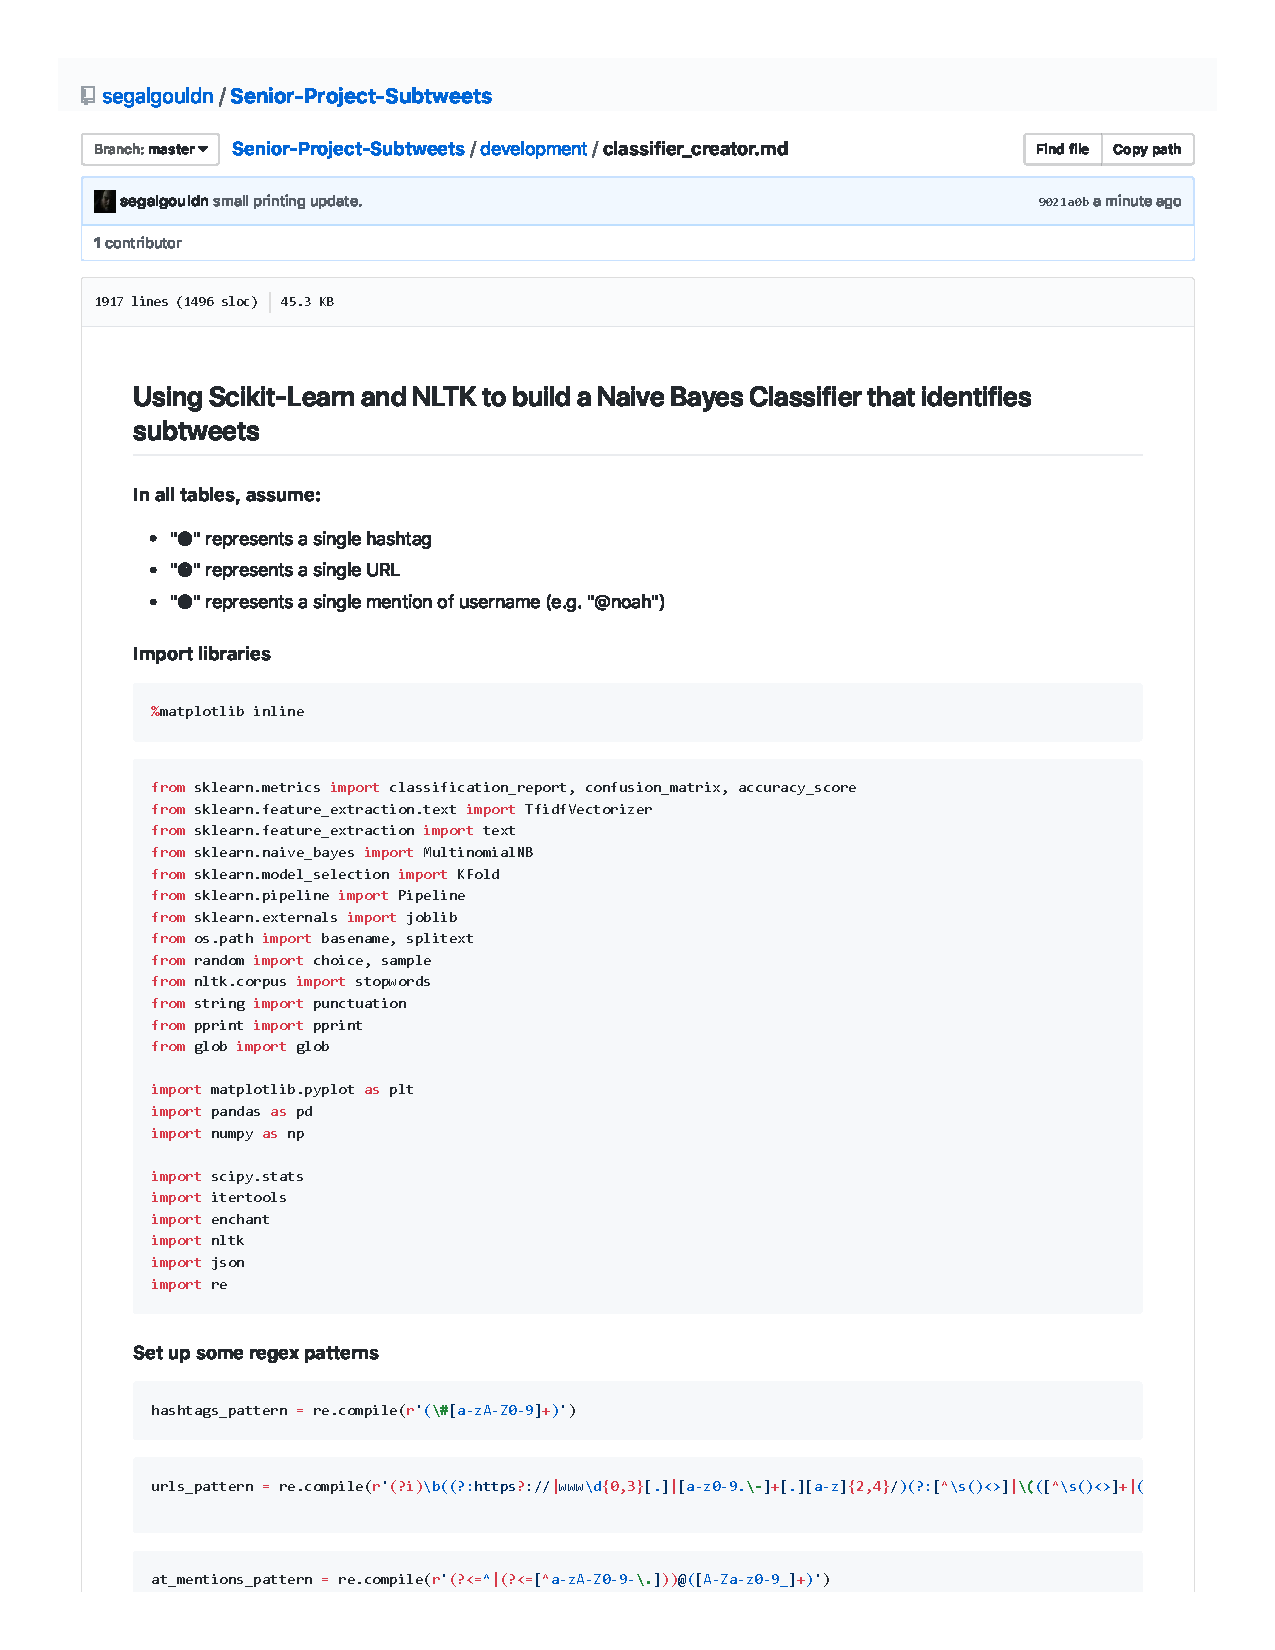
\includepdf[pages=-]{../classifier_creator.pdf}

\chapter{live\_subtweets\_classifier.ipynb}
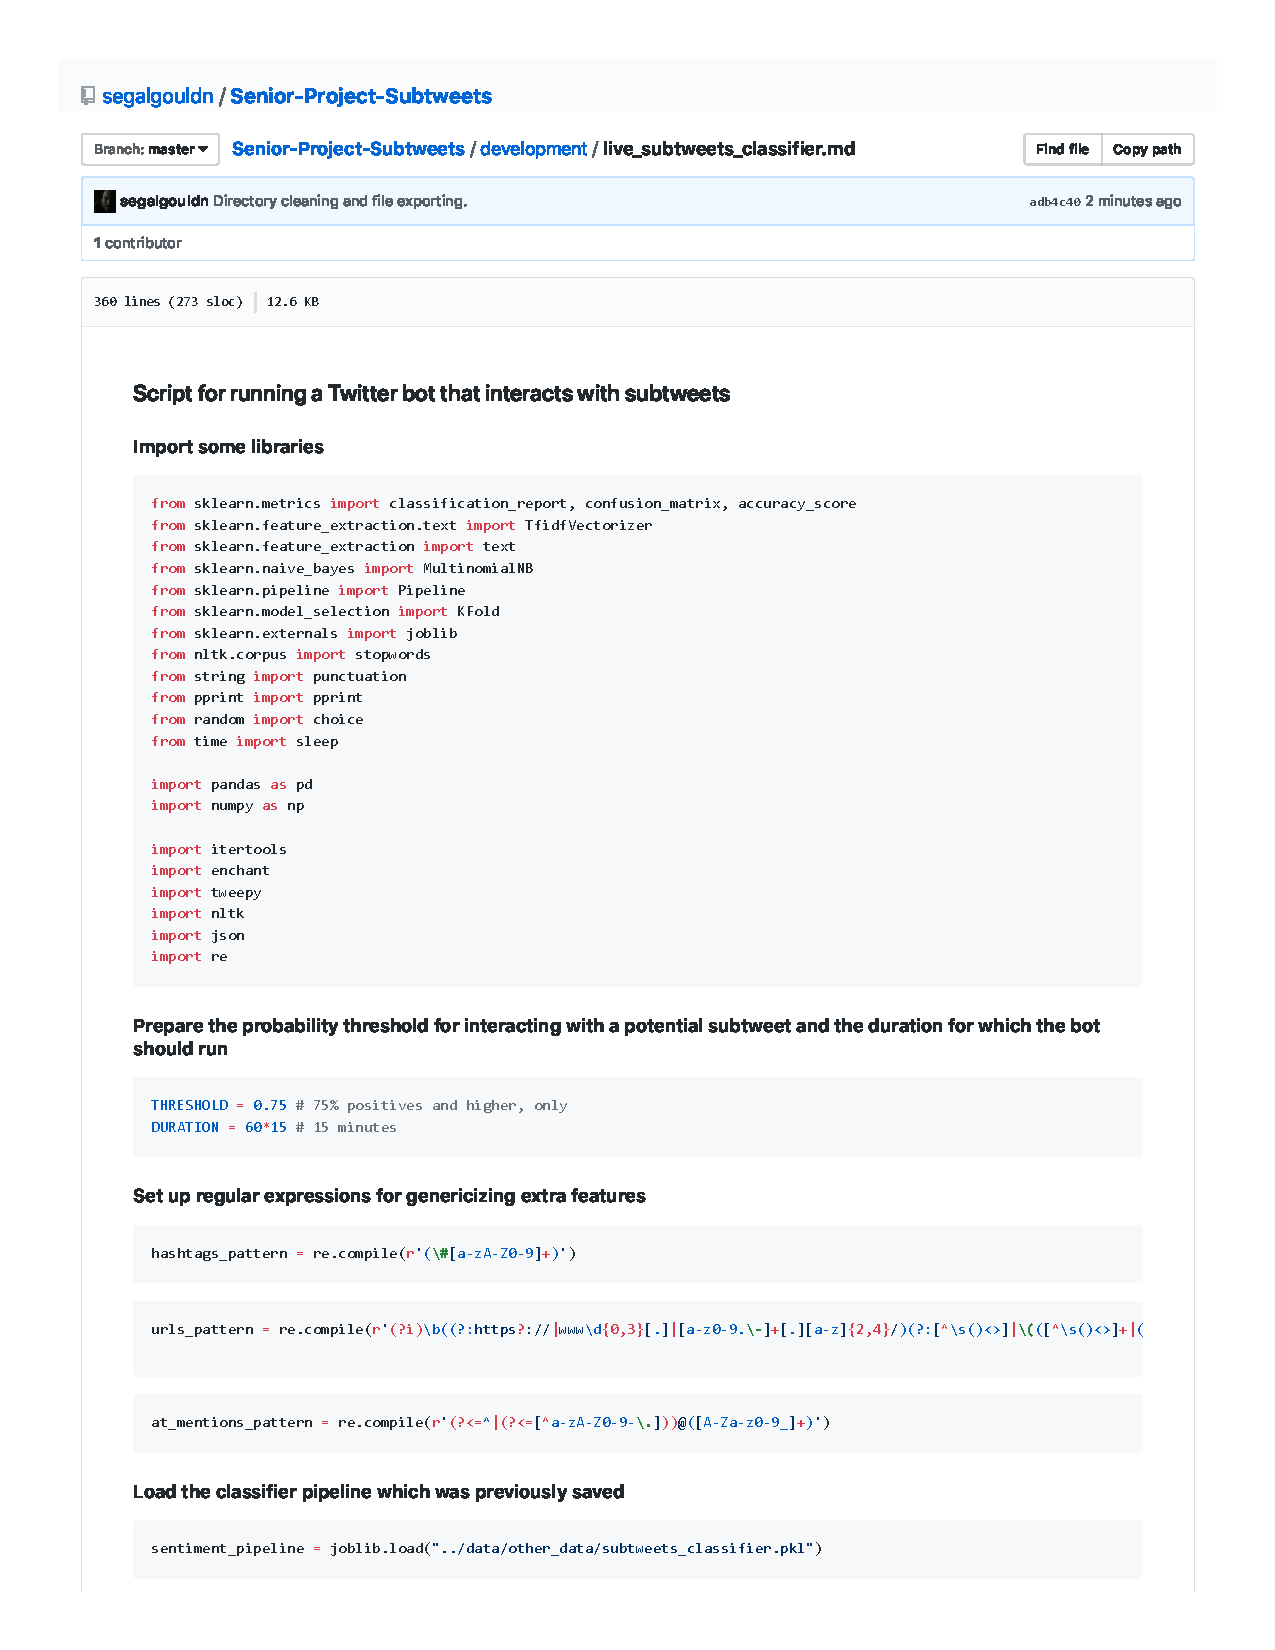
\includepdf[pages=-]{../live_subtweets_classifier.pdf}


\end{appendices}

\end{document}

% end of file bardproj_template.tex
